\centering
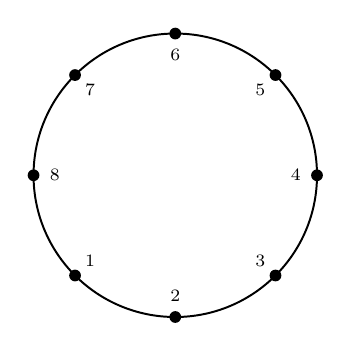
\begin{tikzpicture}[font=\scriptsize, node/.style={circle,thick,draw},
	l_2/.style={line width =0.25mm},
	scale=0.9, transform shape]
	\draw[l_2] (2,0) arc (0:360:2);	
	% equidistant points and arc
	\foreach \x [count=\p] in {0,...,7} {
		\node[shape=circle,fill=black, scale=0.5] (\p) at (\x*45-135:2) {};
	};
	\foreach \x [count=\p] in {0,...,7} {
		\draw (225 + \x*45:1.7) node {\p};
		%				\draw (-30-\x*60:2.4) node {$\bar{\p}$};
	}; 
%	\node (bottom) at (0, -2.8) {};
\end{tikzpicture}
